\documentclass[11pt]{article}
\usepackage{amsmath}
\usepackage{amsfonts}
\usepackage{color}
\usepackage[hidelinks]{hyperref}
\usepackage{graphicx}
\usepackage{listings}
\usepackage{algorithm,algpseudocode}

\title{A Study of the JPEG Compression Standard}
\author{Wenfeng Luo, 18214551}
\date{}

\begin{document}
\maketitle

\section{Introduction}
JPEG is one of the most commonly used lossy compression method for digital images on the World Wide Web. Not surprisingly, JPEG also enters the list of The Top 10 Algorithms \cite{c04} in Applied Mathematics. You're probably already familiar with it since many of the images downloaded from the INTERNET end with the file extension, either jpg or jpeg. In fact, JPEG stands for Joint Photographic Experts Group, which created the compression standard back in 1992. Before we study JPEG in any detail, we first briefly touch a few salient features of the compression standard.

JPEG makes use of some inherent limitations in the human vision system to achieve a higher compression rate. Specifically, our vision system is not sensitive to extremely fine-grained details, which makes it possible to perform a screening procedure to separate the important components from the not so important ones. Then, we could just drop those less important components without causing perceptible loss in image quality.

Since we effectively throw away a lot of the information, JPEG is a lossy compression method, which means that we can not fully recover the original image. However, JPEG is highly customizable and hence allows the user to decide a desired level of quality when it comes to different applications.

As an example, Fig. \ref{effect_of_q} demonstrates the famous Lena image under different quality factor $qf$. (The usual default setting is $qf=75$). 

In the subsequent sections, we will dive into the technical details in the JPEG standard. Section \ref{prelim} prepares the readers with some necessary preliminaries to fully understand the JPEG compression procedure; Section \ref{jpeg_standard} studies JPEG in greater detail, including all the process involved during compression; Section \ref{conclusion} ends this paper with a conclusion.
\begin{figure}
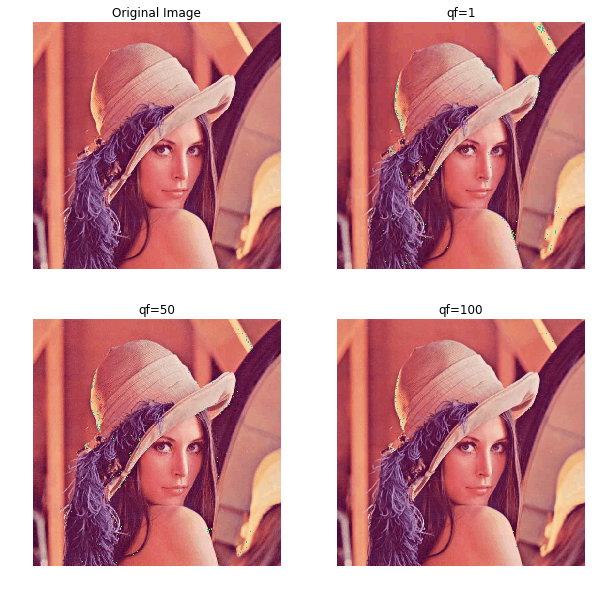
\includegraphics[width=\textwidth]{images/effect_of_q.png}
\caption{The Famous Lena Image Displayed under Different Quality Factor}
\label{effect_of_q}
\end{figure}
%1. One of the mostly used image format on internet.
%2. 3 observations behind the JPEG standard
%3. Lossy compression method
\section{Preliminaries}\label{prelim}
%\subsection{Differential Pulse Code Modulation}
\subsection{Discrete Cosine Transform}\label{dct}
Discrete Fourier Transform (DFT) is a widely used in signal processing to perform de-correlation of the inputs. Despite its effectiveness, DFT involves the manipulation of complex numbers, which are rarely anticipated in real life applications. Fortunately, Discrete Cosine Transform (DCT), simply a mathematic reformulation of DFT, is able to operate only with the real numbers and thus has gained tremendous popularity in daily applications. We'll first discuss the one-dimensional DCT and then the two-dimension DCT that is actually used in JPEG compression.

\textbf{One-Dimensional DCT} Since DCT is a linear transformation of the input signal so we could write it as a matrix multiplication. Denote the input signal as $f\in R^{n}$ and the corresponding output $\hat{f}\in R^n$ in the frequency domain. The transform matrix $C$ is shown below
\begin{equation}
C = \sqrt{\frac{2}{n}}\begin{bmatrix}
\frac{1}{\sqrt{2}} & \frac{1}{\sqrt{2}} & \cdots & \frac{1}{\sqrt{2}} \\
\cos\frac{\pi}{2n} & \cos\frac{3\pi}{2n}  & \cdots & \cos\frac{(2n-1)\pi}{2n}  \\
\vdots & \vdots & \cdots& \vdots \\
\cos\frac{(n-1)\pi}{2n} & \cos\frac{(n-1)3\pi}{2n}  & \cdots & \cos\frac{(n-1)(2n-1)\pi}{2n}  \\
\end{bmatrix}
\end{equation}
where the coefficient $\sqrt{\frac{2}{n}}$ is a scaling factor to form orthonormal basis. So the forward DCT is given by
\begin{align}
\hat{f} = Cf
\end{align}
Since $C$ is a orthogonal matrix, it's easy to recover the original input signal $f$ by making use of the fact that the inverse of $C$ is its transpose. And the following equation gives the inverse DCT
\begin{align}
f = C^{-1}\hat{f}=C^T\hat{f}
\end{align}

\textbf{Two-Dimensional DCT} Basically, 2-D DCT just performs 1-D DCT twice, first along the vertical axis and then along the horizontal axis. Suppose we are given a 2-D input signal $F\in R^{n\times n}$, the forward 2-D DCT is given by
\begin{align}
\hat{F} = C(CF)^T
\end{align}
And similarly, the inverse 2-D DCT is
\begin{align}
F = (\hat{F}C)^TC
\end{align}
\subsection{Huffman Coding}
Huffman Coding was a lossless data compression algorithm, which was first proposed by Huffman back in 1952 \cite{c03} and have since achieved great success in many important applications, such as fax machines and JPEG. Based on the fact that not all the characters transmitted appear equally frequent, Huffman Coding adopts a variable length coding scheme such that those characters with high frequency will be assigned to a  shorter bit pattern than those with relatively low frequency. Compared to the fixed-length 8-bit ASCII coding, some of the characters will have codes greater than 8 bits while the others may have codes lower than 8 bits, but the number of bits per character in average is lower than 8.

There are mainly two major parts in Huffman coding
\begin{enumerate}
\item Build a Huffman Tree from the input characters;
\item Traverse down the Huffman Tree and assign codes to characters.
\end{enumerate}
The following steps specify how to build the Huffman Tree using a priority queue. The algorithm needs only the frequency $f$ of each character as input.
\begin{enumerate}
\item Create a leaf node for each unique character and build a min heap of all leaf nodes. Initially, the least frequent character is at the top of the heap.
\item Pop out two nodes A and B ($f_A < f_B$) with the minimum frequency from the min heap.
\item Create a new internal node whose frequency is the sum of the frequency of node A and B. Then make node A as its left child and node B as its right child. Insert this node to the min heap.
\item Repeat step 2) and 3) until only one node is left in the heap. The remaining node is the root of the Huffman Tree, which is a complete binary tree.  
\end{enumerate}
After the construction procedure, each character (only) appears in the leaf node of the Huffman tree. The path from the root to each leaf node is the bit pattern for each character with 0 going to the left and 1 going to the right. Fig. \ref{huffman_tree} shows a constructed Huffman Tree. The corresponding codes for this Huffman Tree are given in table \ref{huffman_code}.
\begin{figure}
	\centering
	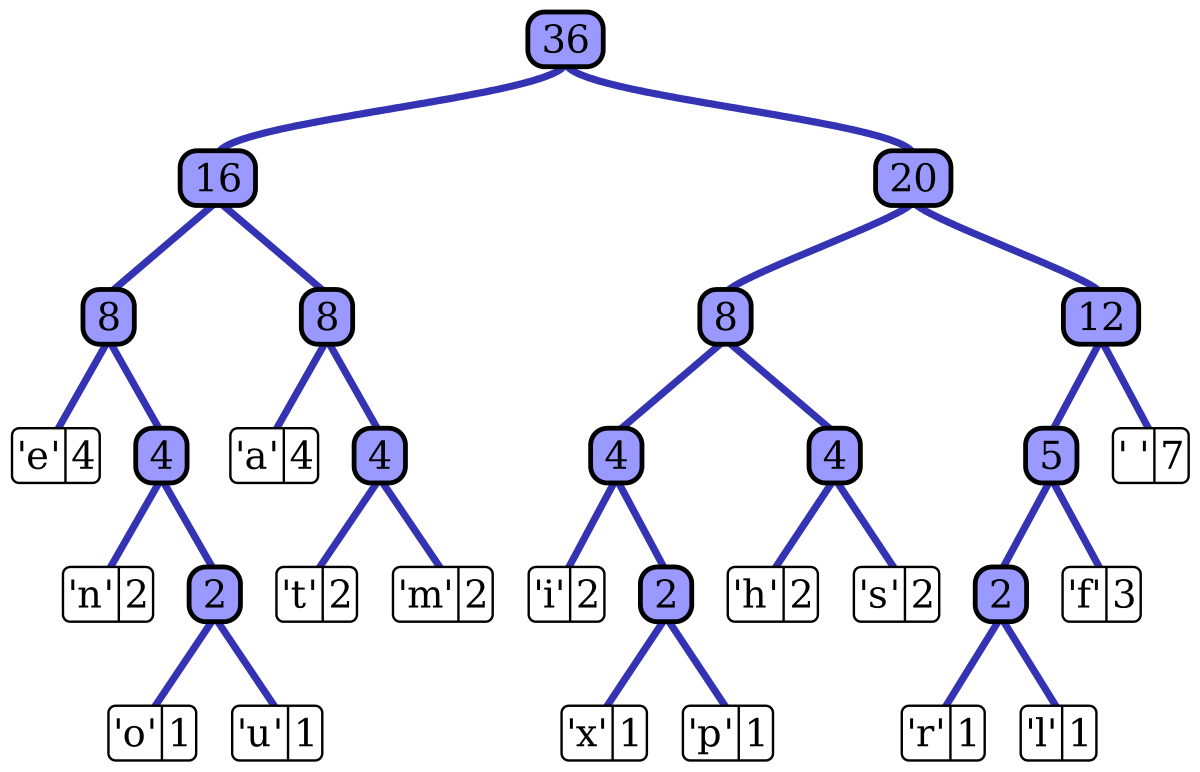
\includegraphics[width=0.5\textwidth]{images/huffman_tree.png}
	\caption{Huffman Tree. The number in the nodes indicates the frequency of the corresponding character. (Image From wikipedia)}
	\label{huffman_tree}
\end{figure}
\begin{table}
	\centering
	\caption{Codes for the Huffman Tree in Fig. \ref{huffman_tree}.}
	\label{huffman_code}
	\begin{tabular}{ccccccccc}
		\hline
		character & e & a & space & n & t & m & i & h\\
		code & 000 & 010 & 111 & 0010 & 0110 & 0111 &1000 & 1010 \\
		\hline
		character & s & f & o & u & x & p & r & l \\
		code & 1011 & 1101 & 00110 & 00111 & 10010 & 10011 &11000 & 11001 \\
		\hline
	\end{tabular}
\end{table}


\section{The JPEG Standard}\label{jpeg_standard}
In this section, we will discuss in details the techniques involved in JPEG compression. The overall encoding process consists of 5 steps, which are color space transformation, down-sampling, Discrete Cosine Transform, \\quantization and entropy coding.
\subsection{Color Space Transformation} 
First, the input image should be converted from RGB into a different color space called $Y'C_BC_R$. It also has three components $Y', C_B\text{ and }C_R$: the $Y'$ component is related to the brightness of a pixel and the other two components represent chrominance. The transformation matrix is given by
\begin{equation}
M = \begin{bmatrix}
0.299 & 0.587 & 0.114 \\
-0.1687 & -0.3313 & 0.5 \\
0.5 & -0.4187 & -0.0813
\end{bmatrix}
\end{equation}
Given a pixel $P = (r, g, b)$, simply by performing matrix multiplication we can obtain the corresponding value $P'$ in the $Y'C_BC_R$ color space
\begin{equation}
\hat{P} = MP
\end{equation} 
\subsection{Downsampling}
Since our vision system is less sensitive to fine color details than to fine brightness, we could reduce the resolution of the $C_B$ and $C_R$ components, usually by a factor of 2 or 3. The commonly used downsampling rates are $4:4:4$ (no downsampling), $4:2:2$ (reduction by a factor of 2 in the horizontal direction) and $4:2:0$ (reduction by a factor of 2 in both directions) \cite{c02}. It is optional and depends on the specific application.

\subsection{Discrete Cosine Transform on Image Blocks}
After subsampling, each individual component is divided into $8\times8$ blocks. One additional operation is that we first subtract each element in the block by 128 to obtain a zero-mean distribution. Then the zero-meaned block is ready to go through the exact same 2-D Discrete Cosine Transform discussed in section \ref{dct}. Note that at this point the image is still fully recoverable since we haven't throw away any information yet, not considering the roundoff error.

\subsection{Quantization}
The quantization step is introduced to reduce those high-frequency contents, which contributes little to the overall image quality. In short, quantization is performed simply by dividing each entry in the frequency domain by a large integer and then round it off to only retain the integral part
\begin{equation}
G(u, v) = \text{round}\left(\frac{F(u, v)}{Q(u, v)}\right)
\end{equation}
where $Q(u, v)$ is an element from the quantization matrix. JPEG standard provides two default quantization matrices, one for luminance component (Fig. \ref{Q} left) and the other for chrominance (Fig. \ref{Q} right).
\begin{figure}
\centering
\resizebox{\textwidth}{!}{  
\begin{tabular}{cc}
\begin{tabular}{rrrrrrrr}
16&11&10&16&24&40&51&61 \\
12&12&14&19&26&58&60&55 \\
14&13&16&24&40&57&69&56 \\
14&17&22&29&51&87&80&62 \\
18&22&37&56&68&109&103&77 \\
24&35&55&64&81&104&113&92 \\
49&64&78&87&103&121&120&101 \\
72&92&95&98&112&100&103&99 \\
\end{tabular} & 
\begin{tabular}{rrrrrrrr}
17&18&24&47&99&99&99&99 \\
18&21&26&66&99&99&99&99 \\
24&26&56&99&99&99&99&99 \\
47&66&99&99&99&99&99&99 \\
99&99&99&99&99&99&99&99 \\
99&99&99&99&99&99&99&99 \\
99&99&99&99&99&99&99&99 \\
99&99&99&99&99&99&99&99 \\
\end{tabular}
\end{tabular}} 
\caption{\textbf{Left} the luminance quantization matrix, \textbf{Right} the chrominance quantization matrix}
\label{Q}
\end{figure}
We can easily control the compression ratio simply by controlling the magnitude of the quantization matrix. In fact, it's done by adjusting the \textit{quality factor} ($qf$), whose value varies from 1 to 100, where $qf =100$ corresponds to the highest quality. Algorithm \ref{alg:scale_q} describes how to obtain the corresponding quantization matrix from the quality factor $qf$. Fig. \ref{jpeg_compress} shows the JPEG compression for a smooth image block. We could see that many of the entries go to zero after the quantization step.
\begin{algorithm}[H] 
	\caption{Scaling Quantization Matrix}
	\label{alg:scale_q}
	\textbf{Input:} quantization matrix $Q$ to be scaled, quality factor $qf$\\
	\textbf{Output:} scaled quantization matrix $Q_x$
	\begin{algorithmic}[1]
		\Statex
		\If{$qf\leq 50$}
		\State{scaling\_factor = (100 - $qf$) / 50;}
		\Else
		\State{scaling\_factor = 50 / $qf$;}
		\EndIf
		\If{scaling factor != 0}
		\State{$Q_x$ = round($Q$ * scaling\_factor);}
		\Else
		\State{$Q_x=Q$;}
		\EndIf
	\end{algorithmic}
\end{algorithm}

\begin{figure}
\centering
\resizebox{\textwidth}{!}{  
\begin{tabular}{cc}
\begin{tabular}{rrrrrrrr}
131&119&116&111&95&103&97&87 \\
131&119&111&106&99&103&97&92 \\
131&119&111&105&99&103&97&92 \\
131&126&116&111&99&97&97&87 \\
131&126&116&111&99&99&97&92 \\
126&119&116&105&103&103&97&92 \\
124&116&116&111&102&97&95&92 \\
123&119&116&111&95&92&87&87 \\
\end{tabular} &
\begin{tabular}{rrrrrrrr}
-168&96&16&9&-3&12&4&-6 \\
5&0&7&9&-3&4&1&-3 \\
-8&-1&-4&-3&2&3&4&-1 \\
5&-3&-1&1&-2&1&1&1 \\
-1&10&-1&-6&-2&3&-3&-4 \\
1&0&-3&-1&0&2&-1&1 \\
-2&-1&0&2&-2&-1&3&0 \\
1&-1&1&-1&2&1&1&-1 \\
\end{tabular} \\
(a) Original pixel value $F(i, j)$ & (b) Domain frequency $\hat{F}(u, v)$ \\
& \\
\begin{tabular}{rrrrrrrr}
-10&9&2&1&0&0&0&0 \\
0&0&0&0&0&0&0&0 \\
-1&0&0&0&0&0&0&0 \\
0&0&0&0&0&0&0&0 \\
0&0&0&0&0&0&0&0 \\
0&0&0&0&0&0&0&0 \\
0&0&0&0&0&0&0&0 \\
0&0&0&0&0&0&0&0 \\
\end{tabular} &
\begin{tabular}{rrrrrrrr}
-160&99&20&16&0&0&0&0 \\
0&0&0&0&0&0&0&0 \\
-14&0&0&0&0&0&0&0 \\
0&0&0&0&0&0&0&0 \\
0&0&0&0&0&0&0&0 \\
0&0&0&0&0&0&0&0 \\
0&0&0&0&0&0&0&0 \\
0&0&0&0&0&0&0&0 \\
\end{tabular}\\
(c) Quantization output $G(i, j)$ & (d) $\tilde{F}(u, v)$\\
& \\
\begin{tabular}{rrrrrrrr}
128&121&111&104&101&97&93&89 \\
130&122&113&106&102&99&94&91 \\
132&124&115&108&104&101&96&93 \\
133&126&116&109&105&102&98&94 \\
133&126&116&109&105&102&98&94 \\
132&124&115&108&104&101&96&93 \\
130&122&113&106&102&99&94&91 \\
128&121&111&104&101&97&93&89 \\
\end{tabular}&
\begin{tabular}{rrrrrrrr}
3&-2&4&7&-6&6&4&-2 \\
1&-4&-2&1&-3&4&3&1 \\
-1&-6&-3&-2&-5&2&1&-1 \\
-2&0&0&2&-7&-5&-1&-7 \\
-2&0&0&2&-7&-3&-1&-2 \\
-6&-6&1&-2&-1&2&1&-1 \\
-6&-7&3&5&0&-2&0&1 \\
-6&-2&4&7&-6&-5&-6&-2 \\
\end{tabular}\\
(e) Recovered image $F'(i, j)$ & (f) Error $\epsilon(i,j) = F(i, j) - F'(i, j)$\\
\end{tabular}}
\caption{Intermediate Outputs During JPEG encoding and decoding.}
\label{jpeg_compress}
\end{figure}

\subsection{Entropy Coding}
Since there are many zero entries after quantization, we could further adopt some lossless coding scheme to obtain a higher rate of compression. Denote the output $G$ from the quantization step. The element on the upper left corner, namely $G(0, 0)$, is called the \textit{DC coefficient} and all the other entries in the matrix $G$ are called the \textit{AC coefficients}.
\subsubsection{Preparation}
Before entropy coding, \textit{DC coefficient} and \textit{AC coefficients} are pre-processed separately: run-length encoding on ACs versus DPCM
on DCs.

\textbf{Run-Length Coding on AC Coefficients} Notice in Fig. \ref{jpeg_compress}(c) there are many zero entries after the quantization step, so \textit{Run-length Coding} (RLC) is very effective in turning matrix G into sets of (\textit{\#zeros skipped, next nonzero value}). RLC is even more effective when we adopt a scanning scheme of \textit{zigzag} to first flatten the $8\times8$ matrix into a 64-d vector, as shown in Fig. \ref{zigzag}. 
\begin{figure}
	\centering
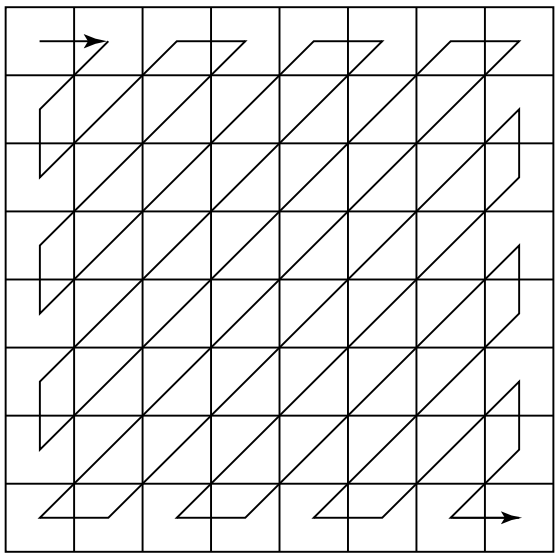
\includegraphics[width=0.5\textwidth]{images/zigzag.png}
\caption{zigzag scan in JPEG\cite{c01}}
\label{zigzag}
\end{figure}
For example, the matrix in Fig. \ref{jpeg_compress}(c) will be flattened as
\begin{align*}
(-10, 0, 9, -1, 0, 2, 0, 0, 0, 1, 0, ..., 0)
\end{align*}
Then we apply RLC to the flattened sequence and have
\begin{align*}
(1, 9), (0, -1), (1, 2), (3, 1), (0, 0)
\end{align*}
where the first element -10 is the DC coefficient and is not taken into consideration. Note the pair $(0, 0)$ at the end, it's a special pair indicating all remaining values are zero and stands for the end-of-block.

\textbf{Differential Pulse Code Modulation on DC Coefficients} There is only one DC coefficient in each $8\times8$ block. Since the DC coefficients represent the average intensity of the block, they could be very large and different. But still the DC coefficients of the adjacent blocks are expected to have similar values due to the continuity inherent in the image, which makes the Differential Pulse Code Modulation (DPCM) a suitable choice for encoding.

Suppose the DC coefficients for the first five blocks are 160, 168, 170, 165, 158, DPCM simply stores the first DC value 160 and the differential value of adjacent ones, which results in the output 160, 8, 2, -5, -7.

\subsubsection{Huffman Coding}
\textbf{Huffman Coding of AC Coefficients} Recall from the previous section the AC coefficients are encoded as pairs of numbers (RUN-LENGTH, VALUE). JPEG goes one step further by decomposing the VALUE into two numbers, namely SIZE and AMPLITUDE, where SIZE is the number of bits to store the actual value AMPLITUDE. Both RUN-LENGTH and SIZE have 4 bits, so they are combined into one single byte to save storage. Note Huffman coding is only applied to the SIZE value.

\begin{tabular}{cc}
(RUNLENGTH+SIZE), & AMPLITUDE) \\
 1 byte & variable bits \\
\end{tabular}

\textbf{Huffman Coding of DC Coefficients} After DPCM, JPEG represents each DC coefficients as (SIZE, AMPLITUDE), where SIZE is the number of bytes to store the AMPLITUDE value. Since the AMPLITUDE value of DC coefficient could vary a lot, only the SIZE is Huffman coded.

\section{Conclusion}\label{conclusion}
This article studies in detail the JPEG standard. The JPEG standard includes both the compression procedure and a set of corresponding exchange formats, such as JPEG File Interchange Format (JFIF), which specify the organization of the bit-stream. The latter is excluded from this article due to the limited length. Readers could refer to the official standard for more technical details.
\bibliographystyle{unsrt}
\bibliography{jpeg}
\end{document}